\section*{Integrais Impróprias}


\subsection*{Intervalo Infinito}
\begin{frame}
\frametitle{ Integrais Impróprias: Intervalo Infinito}
% 

\uncover<1->{Vimos que a integral definida de uma função {\color{blue}positiva} representa a área abaixo de seu gráfico. Analisando o gráfico da função $\dps\frac{1}{x^2}$ quando $x\in[1,+\infty)$ somos levados a pensar que a região sob o gráfico tem {\color{red}área ``infinita''}. }
\bigskip

Sabemos que 
 \[\int\frac{1}{x^2}dx=-\frac{1}{x}+c. \]
 Porém não faz sentido aplicar o Teorema Fundamental do Cálculo.
 \bigskip
 
 
% 
\end{frame}

\begin{frame}[label=improprias]
Entretanto, para cada $t\in(0,1)$ podemos calcular 
 \[\int_1^t\frac{1}{x^2}dx=1-\frac{1}{t}.\]   
 \begin{center}
 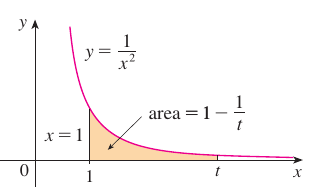
\includegraphics[scale=.7]{impropria1.png}
 \end{center}
Portanto faz sentido aplicar o limite quanto $t\to +\infty$ e podemos definir a {\color{red} área da região} por
\[\int_1^\infty \frac{1}{x^2}\, dx=\lim\limits_{t\to+\infty} \int_1^t\frac{1}{x^2}\, dx=\lim\limits_{t\to \infty} \left(1-\frac{1}{t}\right)=1.\]
\end{frame}



\begin{frame}[label=improprias]
\frametitle{ }
 

\uncover<1->{\begin{defin} \begin{enumerate}[a]
\item Se $\dps\int_a^{{\color{red} b}} f(x)dx$ existe para cada número ${{\color{red}b}}\geq a$, então definimos
\[\int_a^{{\color{red}+\infty}}f(x)dx:=\lim_{{\color{red}b\to+\infty}}\int_a^{{\color{red} b}} f(x)dx.\]


\item Se $\dps\int_{{\color{red}a}}^b f(x)dx$ existe para cada número ${\color{red}a}\leq b$, então definimos
\[\int_{{\color{red}-\infty}}^{b}f(x)dx:=\lim_{{\color{red}a\to -\infty}}\int_{{\color{red}a}}^b f(x)dx.\]


As integrais acima são ditas \dt{impróprias}. Se os limites existem dizemos que as integrais impróprias {\color{blue}convergem} e  se os limites não  existem dizemos que elas {\color{red}divergem}.

\end{enumerate}
\end{defin} }

 
\end{frame}

\begin{frame}
\frametitle{ }
 

\uncover<1->{\begin{defin} Se $\dps \int_{-\infty}^{b}f(x)dx$ e $\dps \int_b^{+\infty}f(x)dx$ são convergentes, então definimos
$$\int_{-\infty}^{+\infty}f(x)dx=\int_{-\infty}^{b}f(x)dx+ \int_b^{+\infty}f(x)dx$$

\end{defin} }



\uncover<1->{\begin{exe}\begin{enumerate}[a]
\item Calcule $\dps\int_{-\infty}^0xe^xdx$

\item Calcule $\dps\int_{-\infty}^{+\infty}\frac{1}{1+x^2}dx$

\end{enumerate}
\end{exe}}

 
\end{frame}



\begin{frame}[label=improprias]
\begin{casa}
 \begin{enumerate}
 \item Determine os valores de $p\in \R$ para os quais a seguinte integral converge
 \[\int_1^{+\infty}\frac{1}{x^p}dx\]
 
 
 \item Calcule o volume do sólido de revolução gerado pela rotação da curva $y=\frac{1}{x}$, quando $1\leq x<+\infty$, em torno do eixo $x$, conhecido como \dt{Trombeta de Gabriel} ou \dt{Trombeta de Torricelli}
 
 
 \begin{center}
 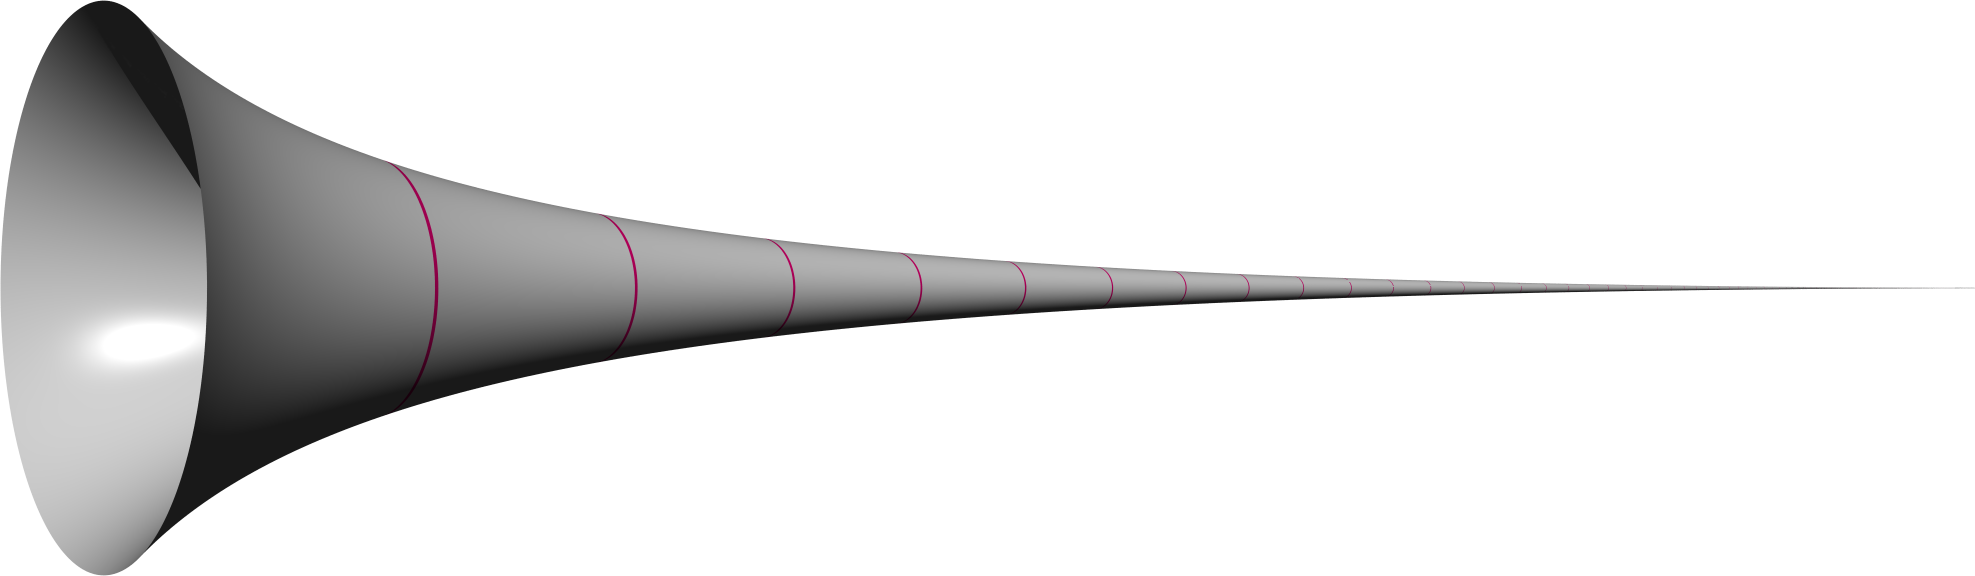
\includegraphics[scale=0.1]{GabrielHorn}
 \end{center}

 \end{enumerate} 
\end{casa}
\end{frame}




\subsection*{Integrando Descontínuo}
\begin{frame}
\frametitle{Integrais Impróprias: Integrando Descontínuo}
% 

Agora, suponha que queremos calcular a área abaixo do gráfico da função $\dps f(x)=\frac{1}{x^2}$ quando $x\in{\color{red}(0},1]$. Sabemos que 
 \[\int\frac{1}{x^2}dx=-\frac{1}{x}+c. \]
 Porém não faz sentido aplicar o Teorema Fundamental do Cálculo, pois a função não está definida em {\color{red}$x=0$}.
\bigskip

De modo análogo ao feito anteriormente, podemos definir a área da seguinte forma
\[\int_{{\color{red}0}}^{1}\frac{1}{x^2}\,dx=\lim_{{\color{red}t\to 0^+}}\int_{{\color{red}t}}^1\frac{1}{x^2}\,dx=\lim_{{\color{red}t\to 0^+}}\left(-1+\frac{1}{t}\right)=+\infty.\]



% 
\end{frame}





\begin{frame}
\frametitle{ }
 

\uncover<1->{\begin{defin} \begin{enumerate}[a]
\item Se $f$ é contínua em $({\color{red}a},b]$ e descontínua em {\color{red}$a$}, então definimos
\[\int_{{\color{red}a}}^b f(x)dx:=\lim_{t\to {\color{red}a^+}}\int_t^b f(x)dx.\]


\item  Se $f$ é contínua em $[a,{\color{red}b})$ e descontínua em {\color{red}$b$}, então definimos
\[\int_a^{{\color{red}b}} f(x)dx:=\lim_{t\to {\color{red}b^-}}\int_a^t f(x)dx.\]


\item  Se $f$ é contínua em $[a,{\color{red}c})\cup({\color{red}c},b]$ e descontínua em {\color{red}$c$}, então definimos
\[\int_a^b f(x)dx:=\int_a^{{\color{red}c}} f(x)dx+\int_{{\color{red}c}}^b f(x)dx.\]

\end{enumerate}
\end{defin} }

 
\end{frame}


\begin{frame}
\frametitle{ }
 

\uncover<1->{\begin{exe}\begin{enumerate}
\item Calcule $\dps\int_{2}^5\frac{dx}{\sqrt{x-2}}$

\item Calcule $\dps\int_0^3\frac{1}{x-1}dx$.

\end{enumerate}
\end{exe} }

\begin{casa}
Calcule 
\[\int_0^1 \log(x)\, dx.\]
\end{casa}


 
\end{frame}


\begin{frame}
\frametitle{Trombeta de Gabriel}
 

\uncover<1->{Podemos encontrar em livros de cálculo que a área de uma superfície gerada pela rotação, em torno do eixo x, do gráfico de uma função $f$ não-negativa definida em $[a,b]$  é dada por
\[S=\int_a^b 2\pi f(x)\sqrt{1+(f'(x))^2}\ dx\]
Com isso temos que a área de superfície da {\color{blue}Trombeta de Gabriel} é dado pela integral 
\[\dps\int_1^{+\infty}2\pi \frac{1}{x}\sqrt{1+\frac{1}{x^4}}dx.\]
}
\end{frame}

\begin{frame}
Note que $\sqrt{1+\frac{1}{x^4}}>1,\ \forall x>0$. Com isso,
\[\int_1^b2\pi \frac{1}{x}\sqrt{1+\frac{1}{x^4}}dx\geq\int_1^b 2\pi \frac{1}{x}dx.\]



\begin{center}
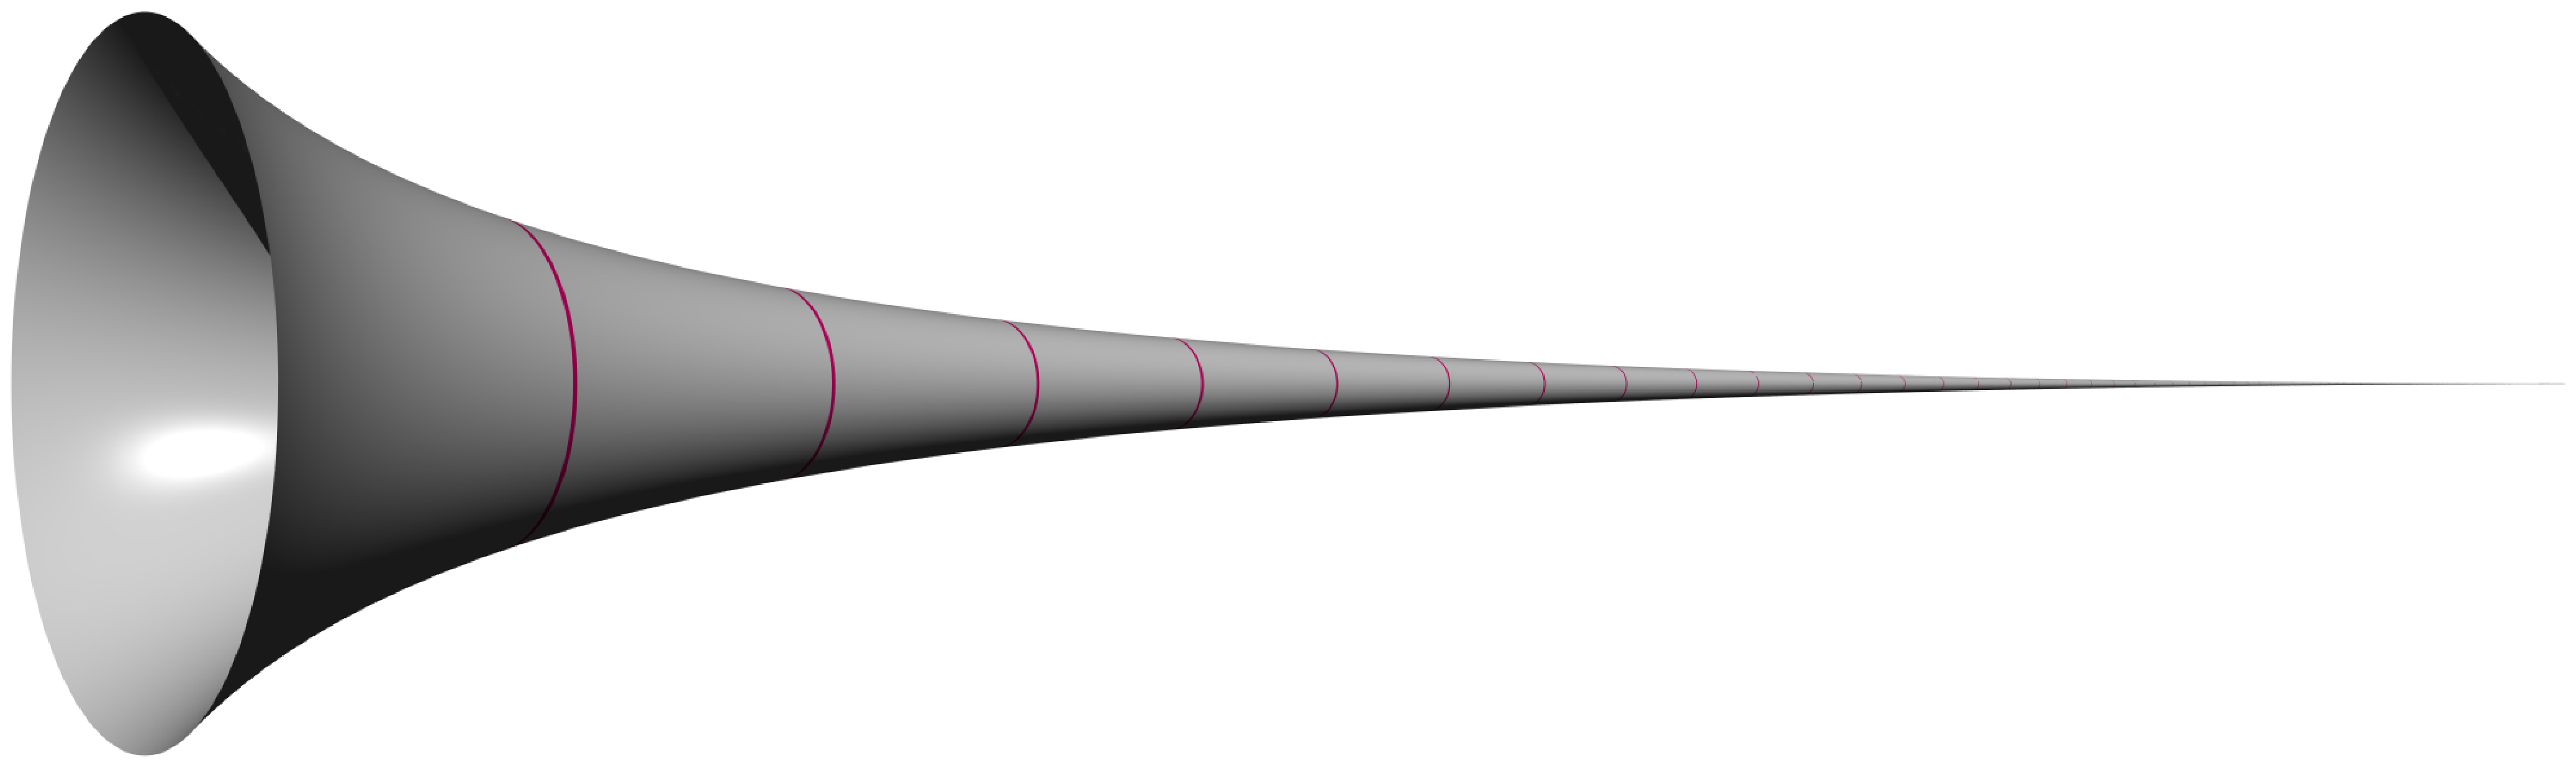
\includegraphics[scale=0.1]{trombeta.eps}
\end{center}

Aplicando o limite deduzimos que a primeira integral diverge. Assim, a trombeta do Anjo Gabriel tem {\color{blue}volume finito} porém {\color{red} área de superfície infinita}, ou seja, O arcanjo poderia encher a trombeta com pouco mais de 3 unidades cúbicas de tinta, mas mesmo que usasse toda a tinta do universo, não poderia pintá-la!!! 

 
\end{frame}


\begin{frame}
\frametitle{ Teste de comparação  }
 

\uncover<1->{Algumas vezes é impossível ou uma tarefa muito difícil calcular o valor exato de uma integral imprópria, mas ainda assim é importante saber se ela é convergente ou divergente

\begin{teo}[Teste de comparação]
Suponha que $f$ e $g$ sejam funções contínuas com ${\color{red}0\leq }\, g(x)\leq f(x)$ para $x\geq a$.
\begin{enumerate}[a]
\item Se $\dps\int_a^b f(x)dx$ é {\color{blue}convergente}, então $\dps\int_a^b g(x)dx$ também {\color{blue}convergente}.
\item Se $\dps\int_a^b g(x)dx$ é {\color{red}divergente}, então $\dps\int_a^b f(x)dx$ também {\color{red}divergente}.
\end{enumerate}
\end{teo}. }

\uncover<1->{O teste também é válido quando um dos extremos do limite de integração é infinito.}



 
\end{frame}


\begin{frame}
\frametitle{ }
 

\uncover<1->{\begin{exe}Decida sobre a convergência das integrais.\begin{enumerate}[a]
\item $\dps \int_1^{\infty}e^{-x^2}dx$
\item $\dps \int_0^{1}\frac{dx}{\sqrt{x+x^3}}$
\end{enumerate}
\end{exe}}



 
\end{frame}



\begin{frame}
\frametitle{Teste de comparação no limite }
 

\uncover<1->{\begin{teo}
Sejam $f$ e $g$  funções \textcolor{red}{positivas} e contínuas em $[a,+\infty)$ tais que
$$\lim_{x\to+\infty}\frac{\textcolor{red}{f(x)}}{\textcolor{blue}{g(x)}}=L.$$
\begin{enumerate}[$i$]
\item Se $0<L<+\infty$, então
as integrais $\dps\textcolor{red}{\int_a^{+\infty}f(x)dx}$ e $\dps\textcolor{blue}{\int_a^{+\infty}g(x)dx}$ são ambas convergentes ou ambas divergentes.
 
 \item Se $L=0$ e $\dps\textcolor{blue}{\int_a^{+\infty}g(x)dx}$ converge, então 
 $\dps\textcolor{red}{\int_a^{+\infty}f(x)dx}$ também converge.
 
\end{enumerate}

\end{teo}}



 
\end{frame}

\begin{frame}
\begin{obs}\begin{enumerate}
\item Se $\dps\lim_{x\to+\infty}f(x)=+\infty$, então  $\dps\int_a^{+\infty}f(x)dx$ diverge.
\item Este teste também é válido para os outros tipos de integrais impróprias, mutatis mutandis.
\end{enumerate}

\end{obs}
\end{frame}



\begin{frame}
\frametitle{ }
 

\uncover<1->{\begin{prop} Seja $f$ contínua em $[a,b)$. Se $\dps\int_a^b|f(x)|dx$ converge, então $\dps\int_a^b f(x)dx$ também converge.
\end{prop}}

\uncover<2->{\begin{exe} Decida sobre a convergência da integrais.
\begin{enumerate}
\item  $\dps \int_1^{+\infty}\frac{dx}{\sqrt{2x^2+5x^3}}$
\item $\dps\int_1^{+\infty}\frac{\sen x}{x^3}dx$
\item $\dps \int_1^{+\infty}\frac{x}{\cosh x}dx$
\end{enumerate}
\end{exe} }

 
\end{frame}
